\chapter{LaRE - Laboratório Remoto Expansível}
\label{Capítulo3}
\begin{center}
    \textit{``All we have to decide is what to do with the time that is given us.''}

    Gandalf
\end{center}

Neste capítulo descreve-se o processo que levou à criação do \acrshort{lare}, a arquitectura de \textit{hardware} e \textit{software}, o motivo das escolhas e a implementação dos circuitos. \textbf{Acho que tem de ser refeito ou complementado}

\section{Contextualização}
\label{sec:contextualização}
Como já foi referido anteriormente (\textbf{ver a referência}) o principal objectivo desta dissertação passa pelo desenvolvimento de um \acrshort{laboratório remoto} para o ensino da electrónica, que visa colmatar (ou resolver) alguns dos problemas que afectam o \acrshort{visir}.

Como referido na Secção \ref{sec:visir}, o \textit{software} do \acrshort{visir} foi lançado sob a licença GNU GPL. No entanto, o \textit{software} de programação do \textit{firmware} do controlador da matriz, que é vendido com a própria matriz, é proprietário da \acrshort{bth}. Quer isto dizer que não pode ser programado ou actualizado por terceiros. Ademais e como já foi referido na Secção \ref{sec:visir}, o equipamento que compreende módulos e placas de instrumentação, é controlado pelo \acrshort{labview}, sendo que os preços das diversas versões variam, aproximadamente, entre os 523€ e os 4300€ anuais \cite{labviewpricing}.

A criação do \acrshort{laboratório remoto} surge como forma de resolver alguns dos problemas que afectam o \acrshort{visir}.

Numa fase mais embrionária, foram feitos alguns testes de controlo de relés com o \gls{arduino} Mega, representado na Figura \ref{fig:arduinomega}, juntamente com um \acrfull{ide} simples desenvolvido em \acrshort{labview}.

\begin{figure}[hbtp]
    \centering
    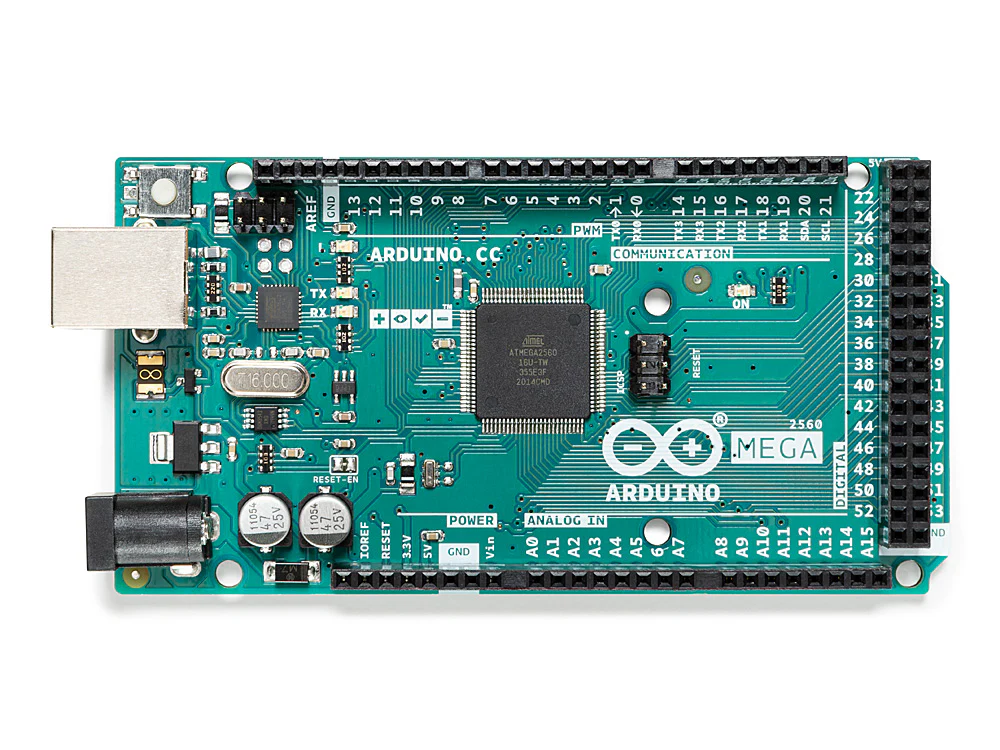
\includegraphics[width=0.6\textwidth]{figures/arduinomega.png}
    \caption{\textit{Arduino} Mega \cite{ArduinoMega}}
    \label{fig:arduinomega}
\end{figure}

No entanto, de forma a ultrapassar o problema levantado pelo elevado preço do \acrshort{labview}, surge um segundo objectivo que se prende com a substituição deste \textit{software} por outro que fosse gratuito e \textit{open source}. A eliminação do \acrshort{labview} implicou a implementação de um servidor. Sendo assim, numa primeira abordagem, foram analisadas algumas opções, tais como: \textit{FastApi}\footnote{\url{https://fastapi.tiangolo.com/}}, \textit{Django}\footnote{\url{https://www.djangoproject.com/}} e \textit{Flask}\footnote{\url{https://flask.palletsprojects.com/en/3.0.x/}}.

As opções analisadas enquadram-se no que se pode chamar \textit{frameworks} ou \textit{micro-frameworks}. Neste caso são todas desenvolvidas para aplicação em \gls{python}.

Uma \textit{micro-framework} é um tipo de \textit{framework} minimalista, que fornece apenas as funcionalidades essenciais para o desenvolvimento de aplicações, sem incluir bibliotecas ou componentes adicionais que não os estritamente necessários. Isso permite a quem desenvolve adicionar apenas as funcionalidades específicas para cada projecto ou aplicação. Daqui resulta um ambiente de desenvolvimento mais leve e flexível \cite{Flask}.
Optou-se, então, pelo \textit{Flask} e as razões da escolha, assim como uma explicação mais detalhada serão apresentadas na Secção \ref{sec:arquitecturasoftware}.

É possível combinar o \gls{arduino} com o \gls{python}, mas isso implicaria uma mudança ao nível do \textit{firmware}, uma tarefa que não é trivial \cite{Arduinopython}. A linguagem nativa do \gls{arduino} é similar ao C++ e o \textit{firmware} instalado foi projectado para interpretar e executar código escrito nesse tipo de linguagem. Para seremos mais rigorosos, o uso do \textit{Python} no \gls{arduino} ou em qualquer outro microcontrolador, faz-se através de \textit{MicroPython}, uma implementação simples e eficiente do \gls{python} que inclui um pequeno subconjunto da bibliotecas padrão e é optimizado para funcionar em microcontroladores e em ambientes limitados \cite{MicroPythondefinition}. Quer isto dizer que todas as bibliotecas usadas na programação da aplicação ou projecto têm de ser carregadas para a memória dos microcontroladores. No caso do \gls{arduino} Mega, uma análise ao \textit{datasheet} \cite{megadatasheet} revela que este tem \SI{256}{Kbytes} reservados para o envio de programas e \SI{8}{Kbytes} de memória \textit{SRAM} reservado para variáveis temporárias.
Além destes problemas de memória e uma vez que é necessário que o \gls{arduino} funcione como servidor, a versão apresentada na Figura \ref{fig:arduinomega} não é adequada.

No mercado, existe o \gls{ESP32}, uma alternativa mais poderosa que o \gls{arduino} e com placa de rede sem fios integrada, tal como é apresentado na Figura \ref{fig:ESP32}. No entanto, este microcontrolador sofre dos mesmos problemas de memória que o \gls{arduino} Mega e da utilização do \textit{MicroPython}. Uma análise ao \textit{datasheet} \cite{esp32datasheet} revela que a memória \textit{flash} varia entre os 4-16 \acrlong{mb}. No modelo ''ESP32-DEVKITC-32E``, que estava disponível para este projecto, o valor é de 4 \acrshort{mb} \cite{diferencaspython}.

Estas limitações não permitem a implementação de um servidor minimamente robusto usando o \gls{arduino} Mega ou o \gls{ESP32}.

\begin{figure}[hbtp]
    \centering
    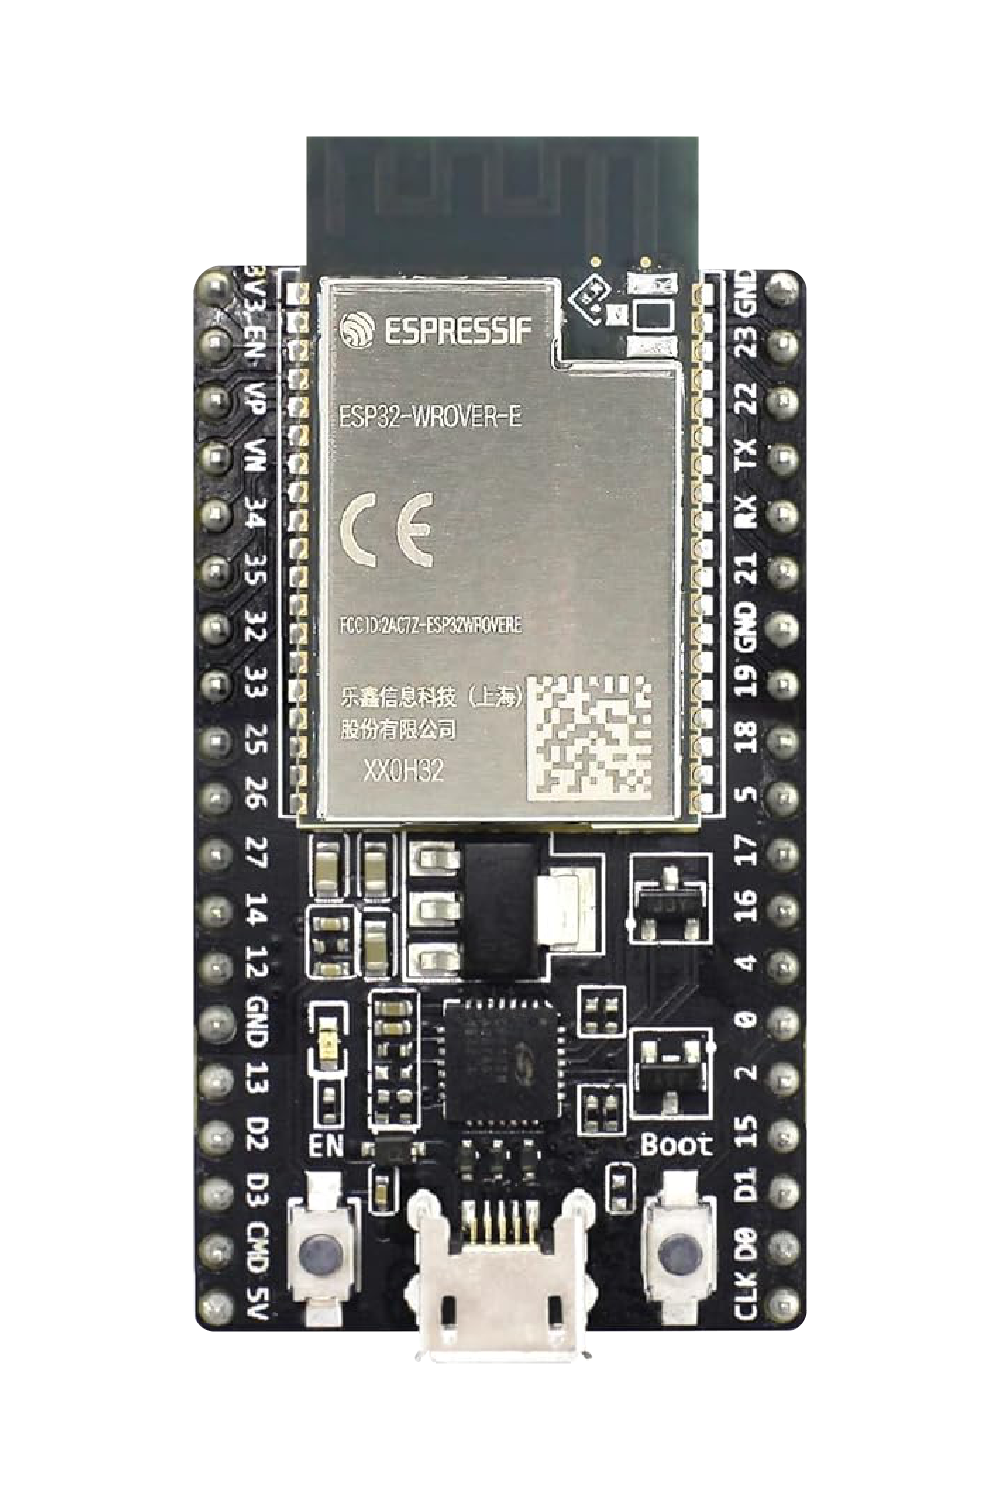
\includegraphics[width=0.4\textwidth]{figures/ESP32-DevKitC_L_0.png}
    \caption{\textit{ESP32} \cite{ESPDevKit}}
    \label{fig:ESP32}
\end{figure}

A escolha seguinte recaiu no \gls{RaspberryPI}, versão 5\footnote{Doravante, sempre que for referido \textit{RaspberryPI}, subentende-se a versão 5.}, que à data da escrita desta dissertação é a versão mais actual, apresentada na Figura \ref{fig:Raspberrypi5}. Este dispositivo insere-se numa gama de pequenos computadores, acessíveis e versáteis que podem ser utilizados para os mais variados projectos. Na Secção \ref{sec:hardware} apresenta-se uma descrição mais detalhada do \gls{RaspberryPI}.

\begin{figure}[hbtp]
    \centering
    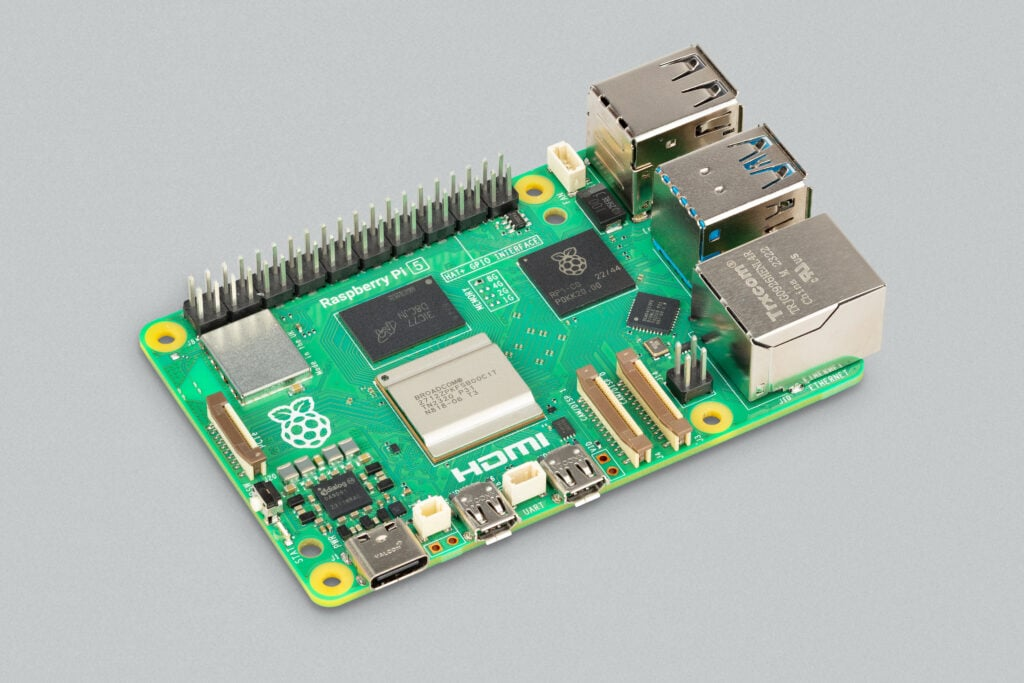
\includegraphics[width=0.6\textwidth]{figures/raspberrypi5.jpg}
    \caption{\textit{RaspberryPI5} \cite{introRaspberrypi5}}
    \label{fig:Raspberrypi5}
\end{figure}

Considerou-se, portanto, que seria uma mais-valia desenvolver um \acrshort{laboratório remoto} com as seguintes características:
\begin{itemize}
    \item \gls{python} como linguagem principal;
    \item \gls{RaspberryPI} como servidor \textit{Flask};
    \item \textit{Interface} com o utilizador desenvolvido em \\
          \acrfull{html}.
\end{itemize}

Estava dado o passo final para o que viria a ser o \acrshort{lare}.

\section{Solução proposta}
\label{sec:solucaoproposta}
Os objectivos principais foram definidos na Secção \ref{sec: Objectivos} e as características gerais definidas na Secção \ref{sec:contextualização}.

Pretende-se que o \acrshort{lare} seja um \acrshort{laboratório remoto} capaz de controlar e comandar um conjunto de experiências electrónicas, assim como efectuar medições de várias grandezas electricas. Para que a solução proposta seja completa e definitiva, falta definir os instrumentos de medida, assim como os circuitos que compõem as experiências.

No contexto desta dissertação, o instrumento de medida sugerido para implementar o \acrshort{lare} foi o \textit{VirtualBench}, modelo VB-8012.

O \textit{VirtualBench} pode ser controlado de duas formas: através do \textit{software} fornecido pela \acrshort{ni} ou através do \textit{pyVirtualBench} \cite{AutomatingVB}. (Apesar de não ser abordado no contexto desta dissertação, existe também a possibilidade de aceder ao \acrshort{virtualbench} através do \acrshort{labview}.)

O \textit{pyVirtualBench} é um \gls{wrapper}\footnote{Este \gls{wrapper} é um \textit{software} de terceiros, suportado e mantido pela comunidade e não é diretamente suportado pela \acrshort{ni}.} que permite controlar o \acrshort{virtualbench} através de uma aplicação \gls{python} \cite{pyvirtualbench}. No entanto, este \gls{wrapper} não é compatível com \textit{Linux}.
Perante este facto, decidiu-se integrar um \acrshort{pc} no \acrshort{lare} - pormenores da instalação do \textit{driver} no \textit{site} da \acrshort{ni} (\href{https://knowledge.ni.com/KnowledgeArticleDetails?id=kA00Z000000kHUFSA2&l=pt-PT}{\textit{link}}) - sendo que todo o peso computacional passaria para o \acrshort{pc} e o \gls{RaspberryPI} controlaria os relés. Esta decisão de o manter como controlador dos relés prendeu-se com o facto de, futuramente, poder haver espaço para uma evolução ao nível da compatibilidade com o \textit{pyVirtualBench}.

A outra forma de controlar o \acrshort{virtualbench} é usando a aplicação disponibilizada pela \acrshort{ni}  e compatível com \textit{Windows}. Esta aplicação faz uma apresentação integrada dos cinco instrumentos apresentados no \acrshort{virtualbench}, como pode ser visto na Figura \ref{fig:leituraohm}. A aplicação também inclui funcionalidades de fluxo de trabalho, como a importação e exportação de configurações de instrumentos e a captura de dados\footnote{\href{https://www.ni.com/en/support/downloads/drivers/download.virtualbench-software.html}{Transferir VirtualBench}}.

De referir que o \acrshort{virtualbench} não pode ser controlado pelo \textit{pyVirtualBench} e pelo \textit{software} simultaneamente.

\begin{figure}[hbtp]
    \centering
    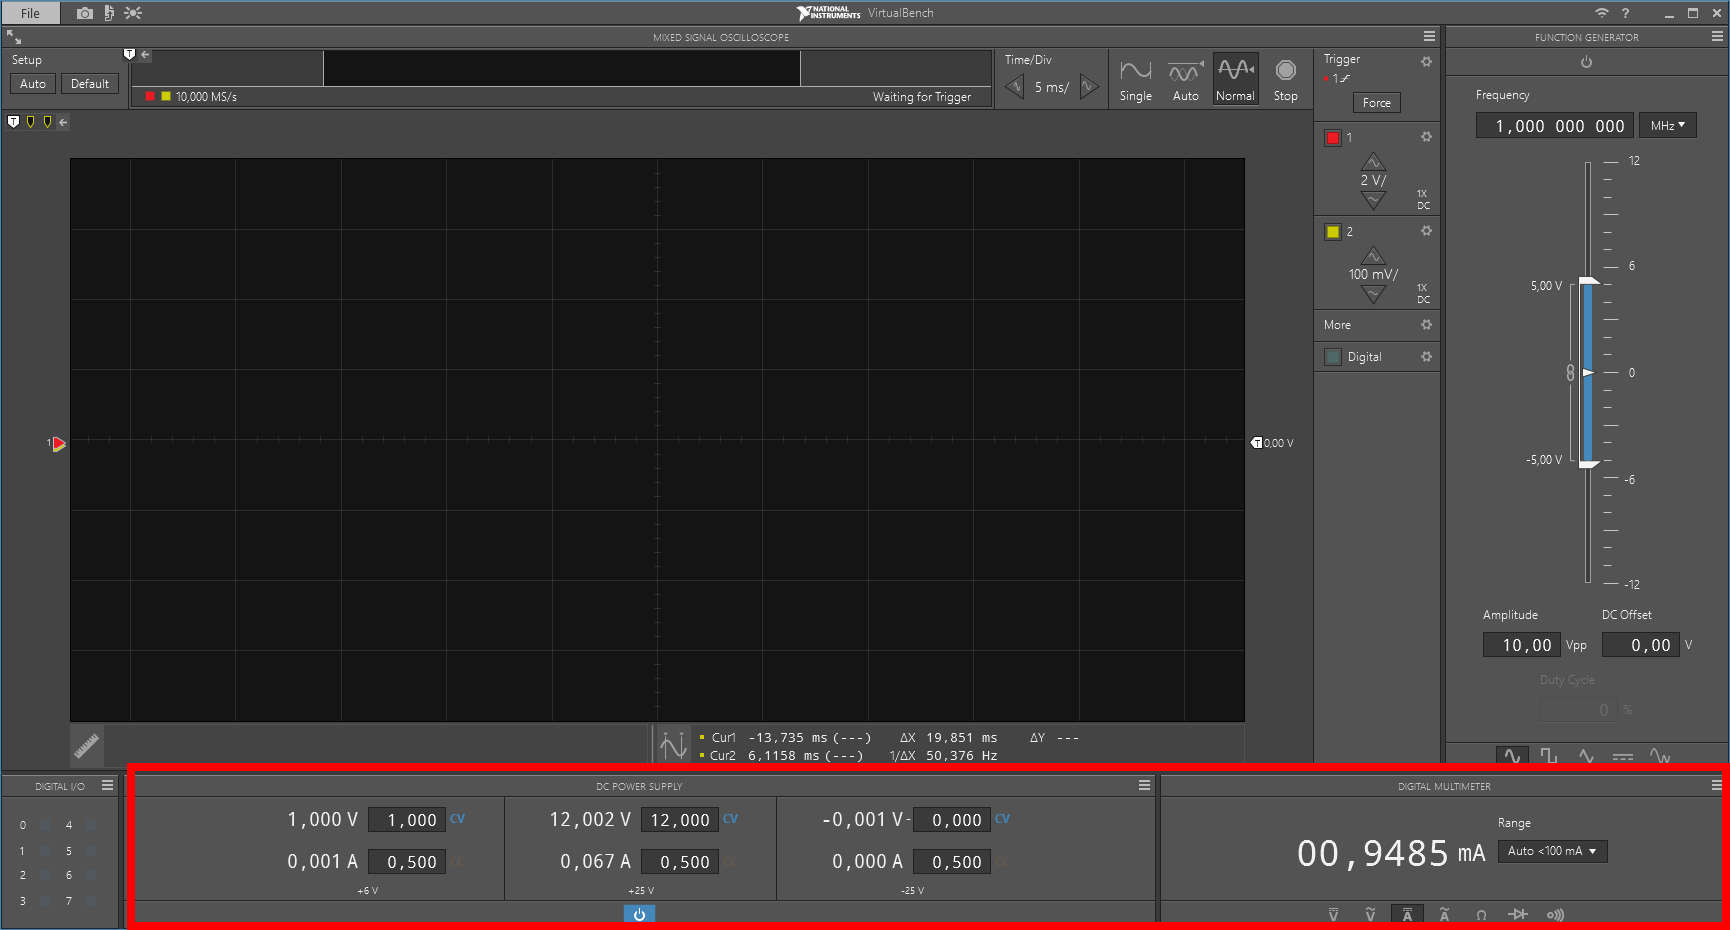
\includegraphics[width=0.9\textwidth]{figures/VB8012-OHM_Exemplo.png}
    \caption{Exemplo do \acrshort{virtualbench} usado como multímetro digital}
    \label{fig:leituraohm}
\end{figure}

As características do \acrshort{laboratório remoto} são, agora, as seguintes:
\begin{itemize}
    \item \gls{python} como linguagem principal;
    \item \acrshort{pc} como servidor \textit{Flask};
    \item \gls{RaspberryPI} como controlador dos relés;
    \item \textit{Interface} com o utilizador desenvolvido em \acrshort{html}.
\end{itemize}

Definidas - de uma forma geral - as soluções de \textit{hardware} e \textit{software}, agora com a integração de um \acrshort{pc} - passou-se ao estudo da arquitectura do \acrshort{lare}.

\section{Arquitectura}
\label{sec:arquitectura}
Como já se viu na Secção \ref{sec:contextualização}, a arquitectura do \acrshort{lare} proposta baseia-se numa estrutura cliente-servidor, suportada ao nível do \textit{hardware} pelo \acrshort{virtualbench}, pelo \gls{RaspberryPI} e um \acrshort{pc} como servidor. Uma representação geral do que será o \acrshort{lare} pode ser vista na Figura \ref{fig:representaçãogerallare}.

\begin{figure}[hbtp]
    \centering
    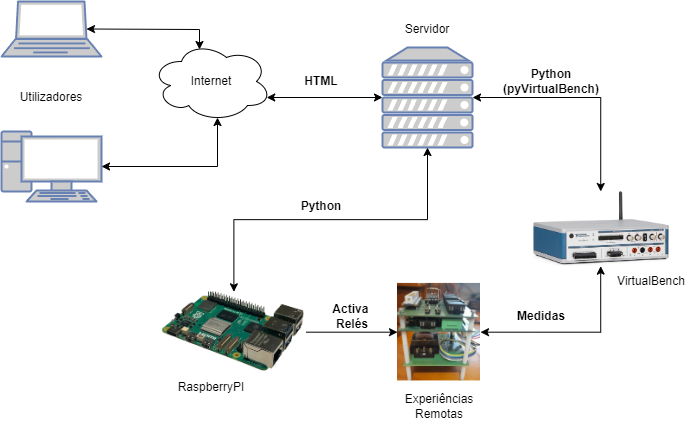
\includegraphics[width=1\textwidth]{figures/arquitectura_ver2.drawio.png}
    \caption{Representação geral do \acrshort{lare}}
    \label{fig:representaçãogerallare}
\end{figure}

Antes de mais, importa clarificar as formas de comunicação entre os diversos dispositivos que compõem o \acrshort{lare}. Tanto o servidor, como o \gls{RaspberryPI} e o \acrshort{virtualbench} têm disponíveis interfaces de rede sem fios e com fios, assim como \textit{interfaces} \acrshort{usb}.

A comunicação entre os diversos dispositivos é feita da seguinte forma:
\begin{itemize}
    \item \textbf{Servidor - \gls{RaspberryPI}}: comunicação via rede sem fios. Em termos de simplicidade de programação, a comunicação entre o servidor e o \gls{RaspberryPI} é feita através da rede sem fios, utilizando \textit{sockets}. Os \textit{sockets} e a \acrshort{api} de \textit{sockets} facilitam a comunicação entre processos em redes, quer estas sejam físicas (ligadas a outras através de fios ou sem fios) ou lógicas (como a rede local de um computador), isto é, permitem o envio de mensagens através de uma rede \cite{Sockets}. O fluxograma de uma chamada ao \textit{sockets} é apresentada na Figura \ref{fig:fluxogramasockets};
    \item \textbf{Servidor - \acrshort{virtualbench}}: comunicação via rede sem fios ou \acrshort{usb}. Entre estes dois dispositivos é, basicamente, indiferente a forma como é feita a comunicação. Isto porque esta parte é gerida pelos \textit{drivers} da aplicação instalada no \textit{Windows}. Independentemente de se utilizar o \textit{pyVirtualBench} ou a aplicação.
    \item \textbf{Controlo de relés e medidas}: O controlo e medição comum às experiência é feito através de ligações directas aos dispositivos.
\end{itemize}

\begin{figure}[hbtp]
    \centering
    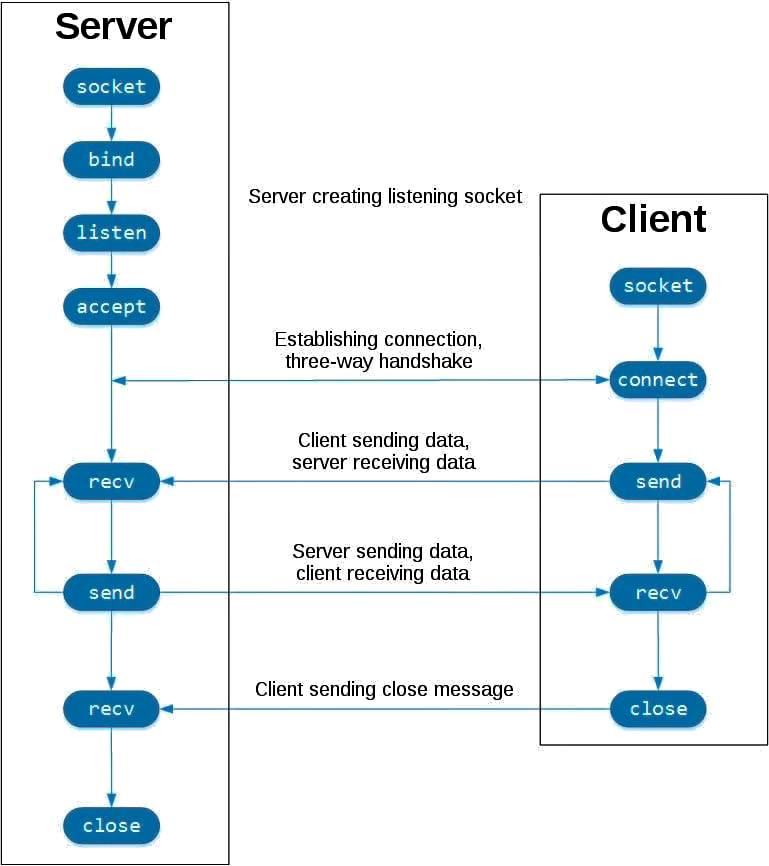
\includegraphics[width=0.7\textwidth]{figures/socketsdiagrama.png}
    \caption{Fluxograma de uma chamada ao \textit{socket} \cite{Sockets}}
    \label{fig:fluxogramasockets}
\end{figure}

Ao nível do \textit{software}, o servidor será implementado no \acrshort{pc} com base no \textit{Flask}, como já foi referido na Secção \ref{sec:contextualização} e \ref{sec:solucaoproposta}, e será descrito com mais pormenor na Secção \ref{sec:arquitecturasoftware}. A comunicação entre o servidor e o \acrshort{virtualbench}, entre o servidor e o \gls{RaspberryPI} e o controlo dos relés é feita em \textit{Python}. A \textit{interface} com o utilizador é feita em \acrshort{html}.

A Figura {\ref{fig:arquitecturalore}} apresenta com mais pormenor a solução implementada no \acrshort{lare}. De uma forma geral, podemos ver como é realizada a comunicação e a troca de informação entre os diferentes dispositivos de \textit{hardware}.

\begin{figure}[hbtp]
    \centering
    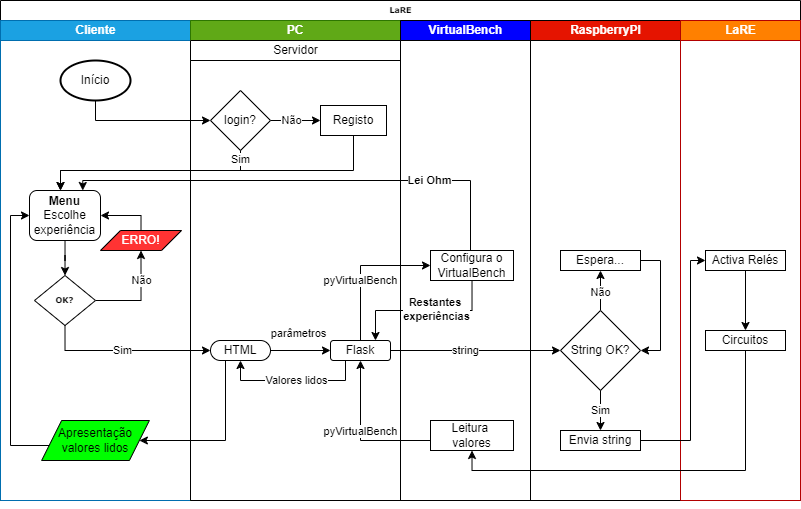
\includegraphics[width=1\textwidth]{figures/Diagrama_SOFTWARE.drawio.png}
    \caption{Arquitectura \acrshort{lare}}
    \label{fig:arquitecturalore}
\end{figure}

\section{Circuitos electrónicos - experiências?}
\label{sec:circuitos}
\textbf{Não sei até que ponto esta secaçõp não se enquadra melhor no hardware}
A escolha dos circuitos teve como base os que estão disponíveis no \acrshort{visir} do \acrshort{isep}, como se pode ver na Figura \ref{fig:circuitosvisir}. Reduzindo os objectivos do \acrshort{lare} à sua forma mais básica, pode afirmar-se que se pretende ``provar um conceito''. Escolhendo experiências com circuitos integrados ou transístores, poderia tornar a implementação desnecessariamente mais complexa e, por conseguinte, com menos experiências. Portanto, o objectivo passará por criar um \acrshort{laboratório remoto} com experiências típicas para a introdução à electrónica e que permitam uma aprendizagem gradual em contexto de sala de aula. E, assim, ``provar o conceito''.

\begin{figure}[hbtp]
    \centering
    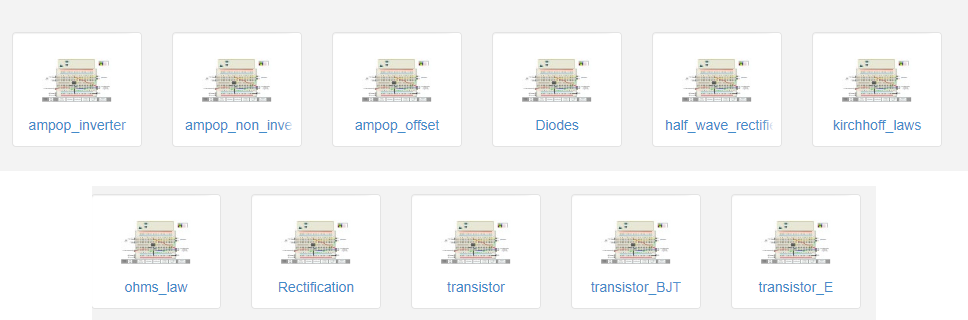
\includegraphics[width=1\textwidth]{figures/visir_ISEP.png}
    \caption{Circuitos \acrshort{visir} - \acrshort{isep} - \textbf{Se calhar retirava a imagem}}
    \label{fig:circuitosvisir}
\end{figure}

Sendo assim, os circuitos que compõem o \acrshort{lare} e satisfazem os critérios definidos em cima são:
\begin{itemize}
    \item Lei de Ohm;
    \item Rectificador de meia onda;
    \item Rectificador de onda completa;
    \item Filtro RC passa-baixo;
    \item Filtro RC passa-alto.
\end{itemize}

\section{Hardware}
\label{sec:hardware}
\subsection{VirtualBench}
Este dispositivo desenvolvido pela \acrshort{ni} integra vários instrumentos e ferramentas de teste, tais como um osciloscópio digital com análise de protocolo, um gerador de formas de onda, um multímetro digital, uma fonte de alimentação \acrfull{cc} programável e E/S digitais num único dispositivo que se liga a um \acrshort{pc}, via \acrshort{usb} ou rede sem fios, como se pode ver na Figura \ref{fig:paineltraseiro}. As principais características deste modelo estão descritas na Figura \ref{fig:paineldianteiro} \cite{datasheetVirtualBench}. A forma como pode ser controlado e configurado já foi abordada na Secção \ref{sec:solucaoproposta}.

\begin{figure}[hbtp]
    \centering
    \centering
    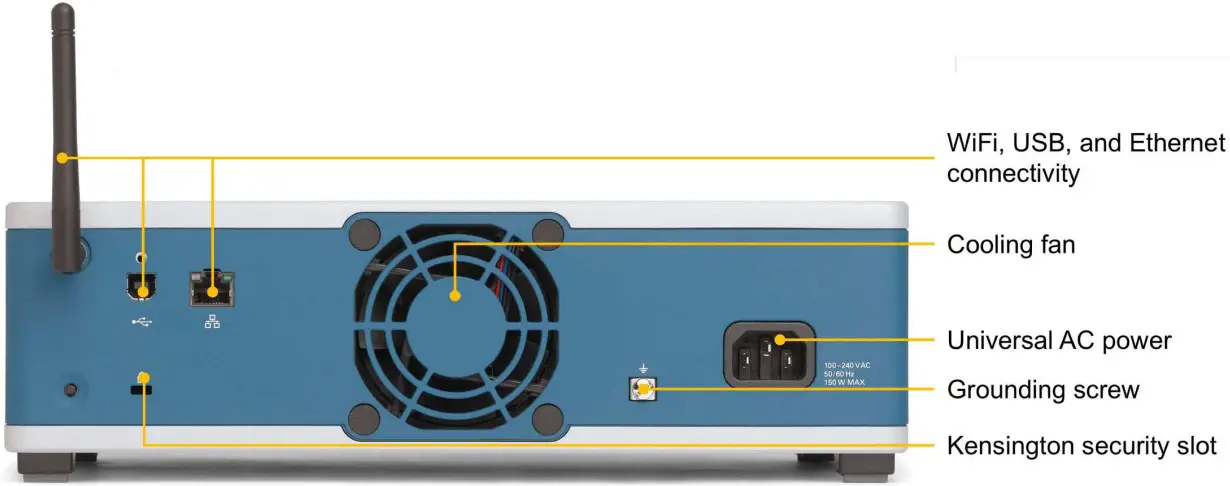
\includegraphics[width=0.7\textwidth]{figures/virtualbench_back-panel.jpg}
    \caption{Painel traseiro \textit{VirtualBench} VB-8012  \cite{datasheetVirtualBench}.}
    \label{fig:paineltraseiro}
\end{figure}

\begin{figure}[hbtp]
    \centering
    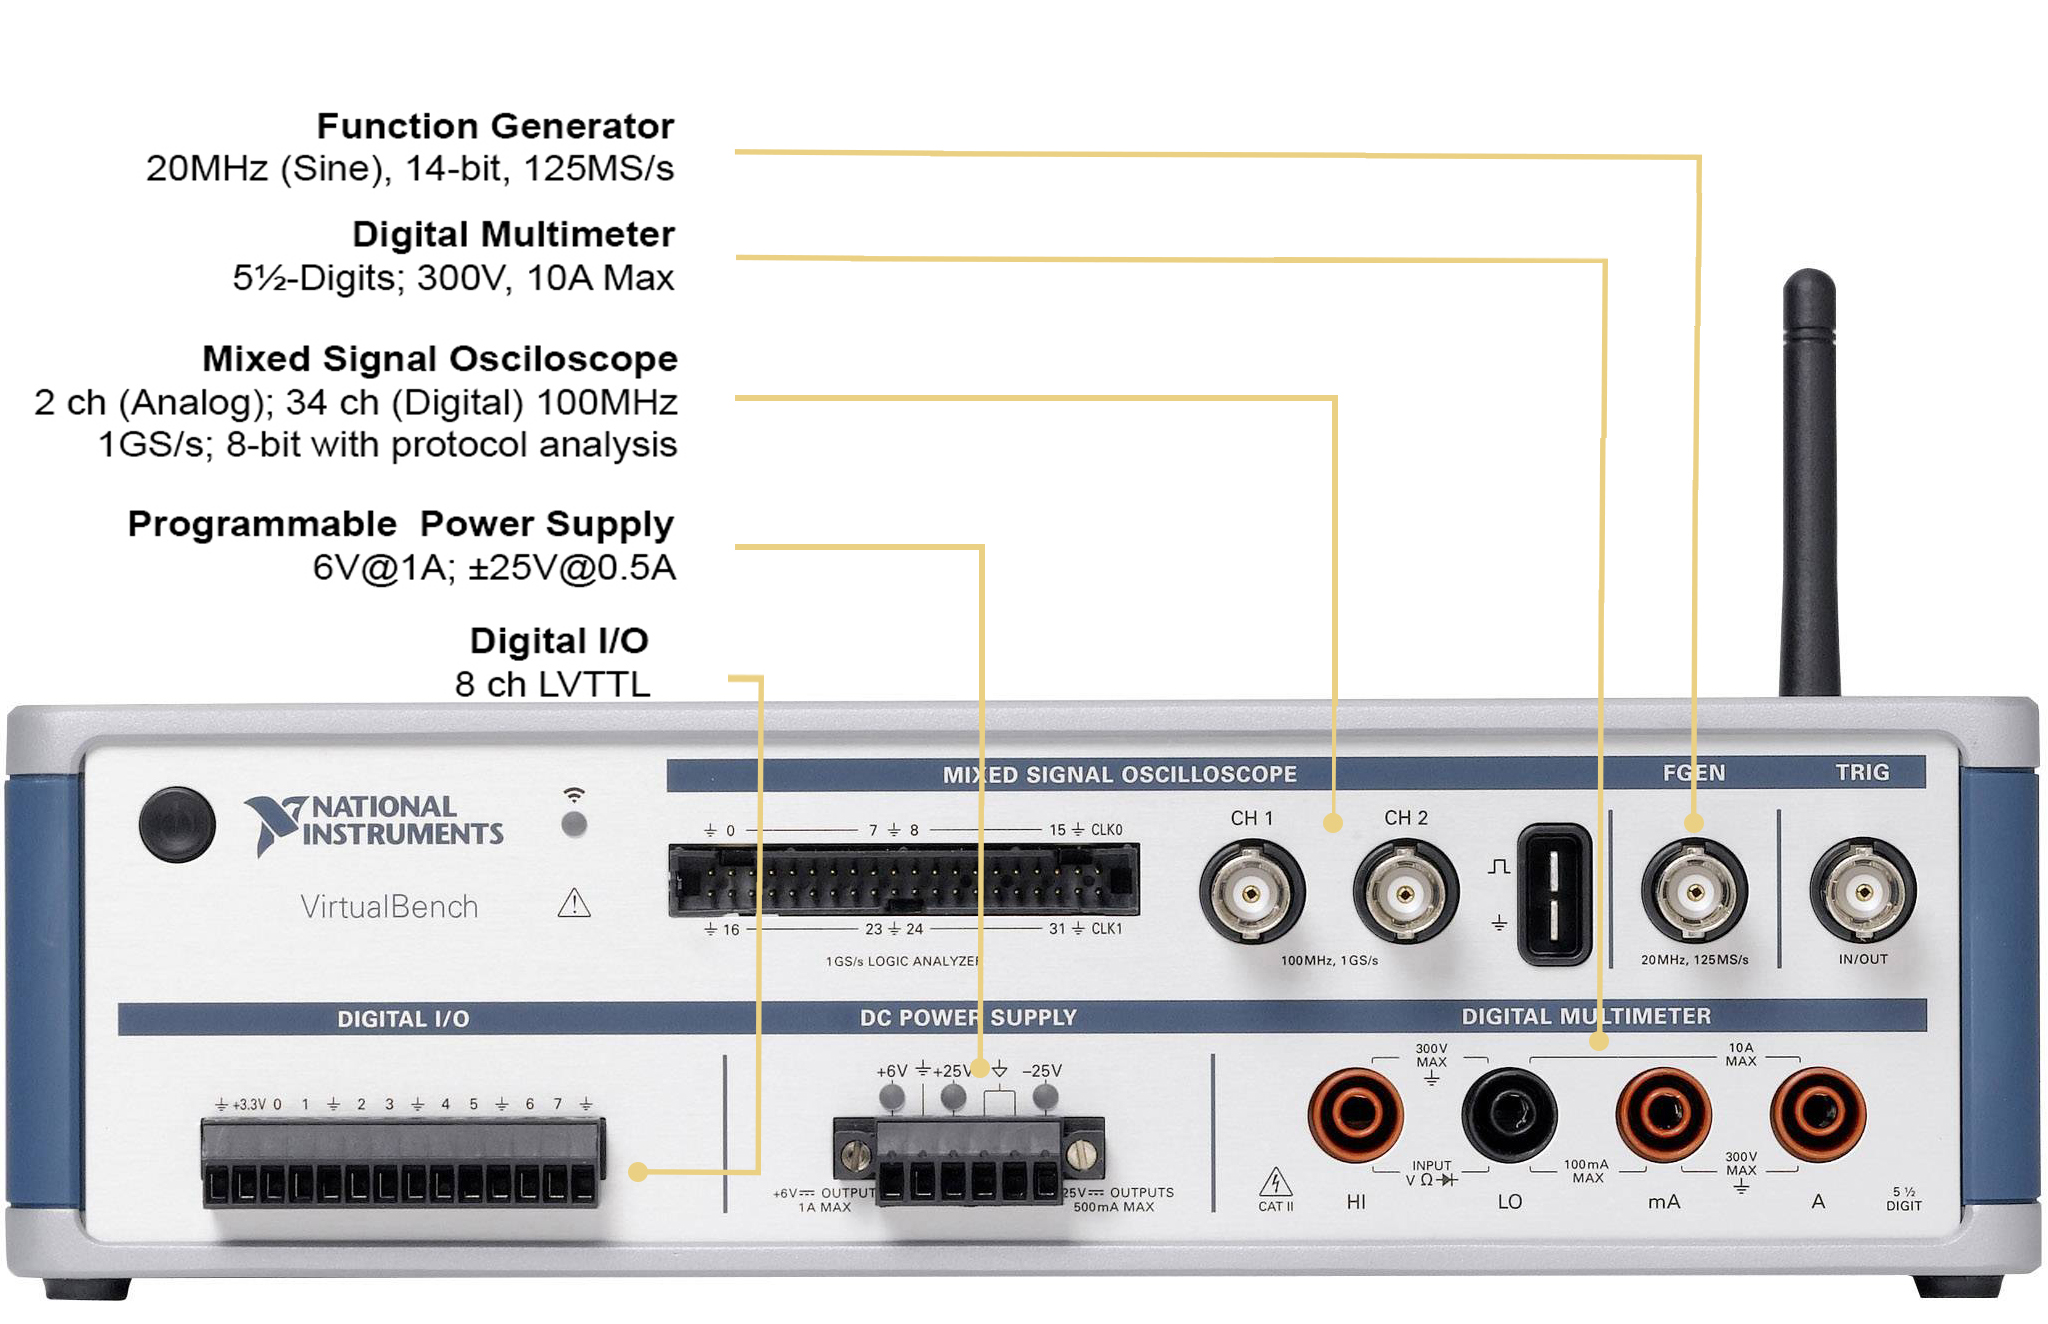
\includegraphics[width=0.7\textwidth]{figures/virtualbench_front-panel.jpg}
    \caption{Painel frontal \textit{VirtualBench} VB-8012  \cite{datasheetVirtualBench}.}
    \label{fig:paineldianteiro}
\end{figure}

%No \acrshort{visir} do \acrshort{isep}, estão disponíveis 11 circuitos, como se pode ver na Figura \ref{fig:circuitosvisir}. Os circuitos que compõem o \acrshort{laboratório remoto} tiveram como base (ou ponto de partida) os que estão implementados no \acrshort{isep}. \textbf{Faz sentido? PROF}

\subsection{Matriz LaRE}
\label{sec:matriz}
Encontradas as soluções de \textit{hardware} e \textit{software}, assim como as experiências a serem implementadas, partiu-se para o projecto da matriz.

Mais uma vez, tomando como base o \acrshort{visir}, como pode ser visto mais pormenor na Figura \ref{fig:visir104}, decidiu-se projectar uma matriz com a dimensão das placas a obedecerem às definidas pela consórcio \gls{pc/104} \cite{PC104}. Este consórcio definiu um padrão que se destaca pelo seu formato compacto e modular. As dimensões mecânicas das placas estão definidas na \textbf{referência ao datasheet - VER COPMO FAZER REFERÊNCIA}.

\begin{figure}[hbtp]
    \centering
    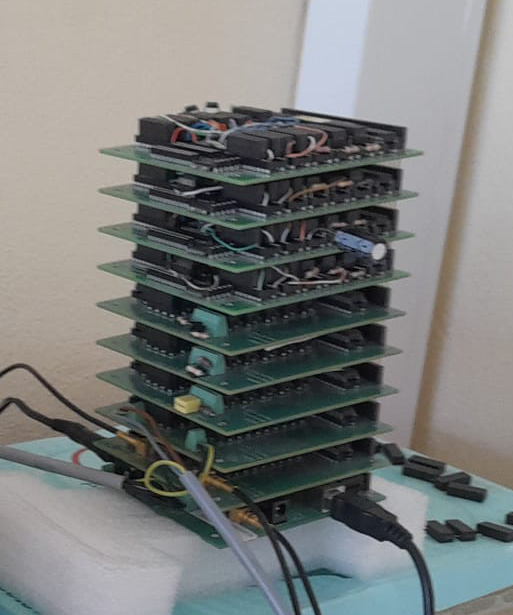
\includegraphics[width=0.3\textwidth]{figures/promenorvisirISEP.png}
    \caption{Placas PC/104 do \acrshort{visir} - \acrshort{isep} - \textbf{Foto com melhor qualidade}}
    \label{fig:visir104}
\end{figure}

\subsection{RaspberryPI}
\label{sec:RaspberryPI}
Como já foi referido na Secção \ref{sec:contextualização}, a ideia inicial passava por utilizar o \gls{RaspberryPI} como servidor e como controlador dos relés, no fundo desempenhando as funções de \acrshort{rlms}.

Em contexto de laboratório estavam disponíveis os modelos PI2 e PI3, algo desactualizados. O PI3 já se mostrou lento nos primeiros testes e, por isso, optou-se pela última versão do \textit{RaspberryPI}.

Esta versão traz várias melhorias e novos recursos, sendo que as principais diferenças de \textit{hardware} para a versão 4B estão representadas na Tabela \ref{Table:diferencasPI4PI5}. No entanto, estas melhorias acarretam um maior consumo de energia e, por isso, é recomendado o uso de arrefecimento activo \cite{Raspberrytech}. Na Figura \ref{fig:pi5dissipador} está representado o \gls{RaspberryPI} usado no \acrshort{lare}.

\begin{figure}[hbtp]
    \centering
    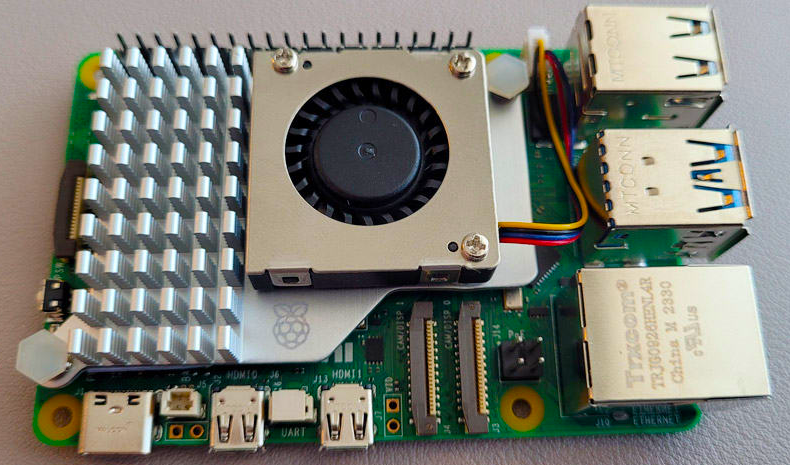
\includegraphics[width=0.7\textwidth]{figures/pi5_dissipador.png}
    \caption{\textit{Raspberry PI5} com dissipador activo utilizado no \acrshort{lare}}
    \label{fig:pi5dissipador}
\end{figure}

\begin{table}[htb]
    \centering
    \caption{Raspberry PI4 \textit{vs Raspberry PI5 - principais diferenças} \cite{Raspberrypi5}}
    \label{Table:diferencasPI4PI5}
    \begin{tabular}{ll}
        \toprule
        Raspberry PI4                                            & Raspberry PI5                                             \\
        \midrule
        \SI{1.8}{\giga\hertz}                                    & \SI{2.4}{\giga\hertz}                                     \\
        \midrule
        VideoCore VI @ \SI{500}{\mega\hertz}, Vulkan 1.0         & VideoCore VII @ \SI{800}{\mega\hertz}, Vulkan 1.2         \\
        \midrule
        LPDDR4-3200 SDRAM até \SI{8}{\giga\byte}                 & LPDDR4X-4267 SDRAM \SI{4}{\giga\byte}/\SI{8}{\giga\hertz} \\
        \midrule
        \SI{5}{\volt}/\SI{3}{\ampere} via USB-C (\SI{15}{\watt}) & \SI{5}{\volt}/\SI{5}{\ampere} via USB-C (\SI{27}{\watt})  \\
        \bottomrule
    \end{tabular}
\end{table}

Comum às versões anteriores, o \gls{RaspberryPI} possui um conector de 40 pinos denominados \acrfull{gpio}s, como se pode ver na Figura \ref{fig:gpio}. Os \acrshort{gpio}s são pinos versáteis e configuráveis e permitem que a placa interaja com uma variedade de componentes eletrónicos e outros dispositivos, como por exemplo, relés, sensores, motores, etc.. Os \acrshort{gpio}s são pinos digitais, isto é, o \gls{RaspberryPI} não possui um \acrfull{adc} interno para ler sinais analógicos. No entanto, pode usar-se um \acrshort{adc} externo, como por exemplo, o MCP3008 ou o módulo ADS1115. Quer isto dizer que só trabalham com duas tensões: \SI{3.3}{\volt} ou \SI{0}{\volt}, correspondendo aos valores lógicos ``1'' ou ``0'', respectivamente.
Dependendo da configuração dos \acrshort{gpio}s - entrada ou saída - estes podem ler ou fornecer as tensões correspondentes aos níveis lógicos desejados. O \gls{RaspberryPI} pode fornecer uma corrente até \SI{16}{\milli\ampere} por cada \acrshort{gpio} ou \SI{50}{\milli\ampere} se combinados \cite{Raspberrytech}.
%No caso extremo de todas os 17 \acrshort{gpio}s estarem activos ao mesmo tempo, a corrente total seria de \SI{272}{\mA}. Nesta situação, a fonte de \SI{3.3}{\volt} colapsava.

Se for fornecida uma tensão superior a \SI{3.3}{\volt} aos \acrshort{gpio}s, o \gls{RaspberryPI} corre o risco de se danificar irremediavelmente.

\begin{figure}[hbtp]
    \centering
    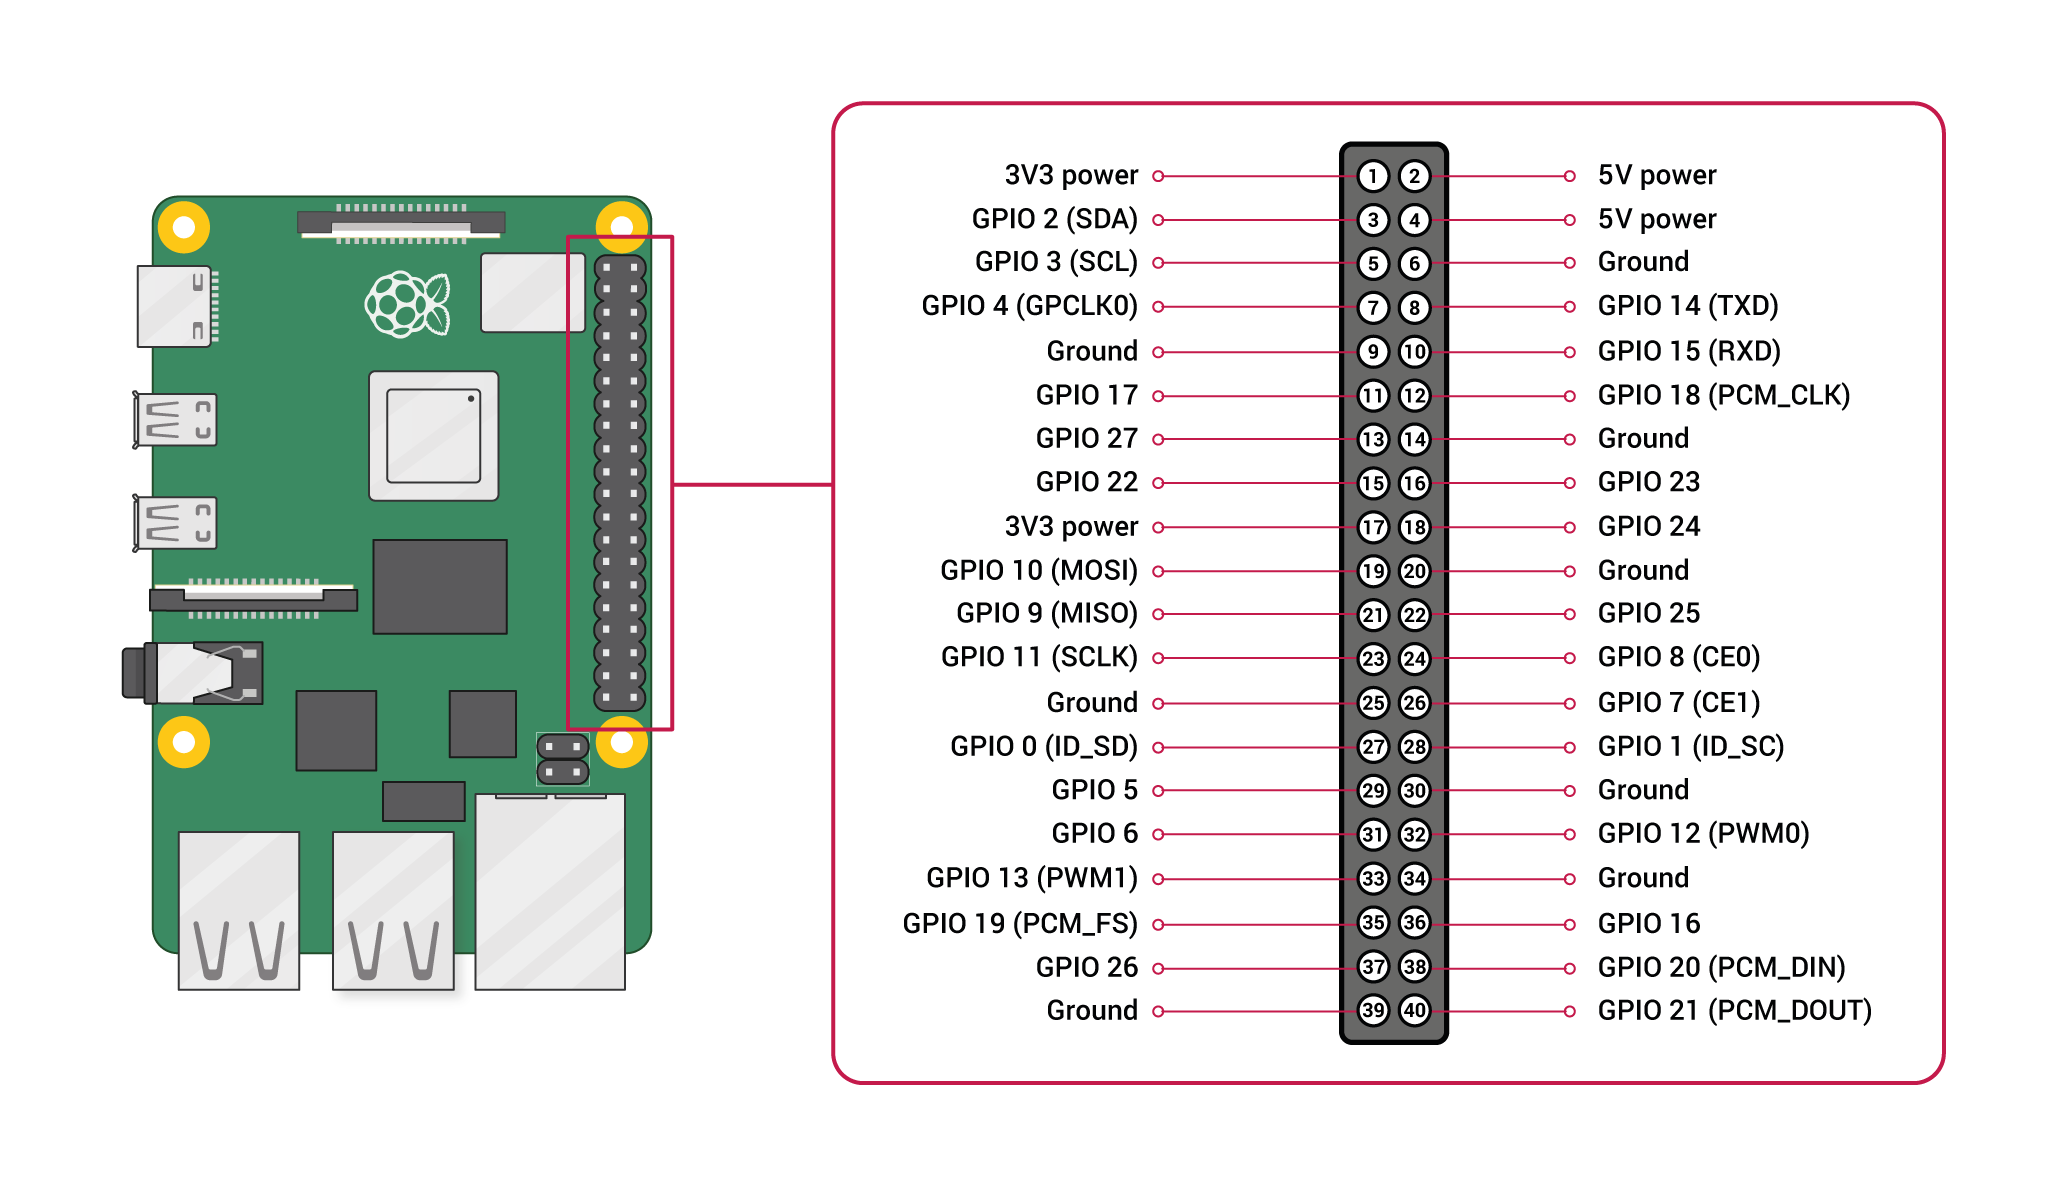
\includegraphics[width=0.7\textwidth]{figures/GPIO-Pinout-Diagram-2.png}
    \caption{\acrshort{gpio}s \textit{RaspberryPI} \cite{Raspberrytech}}
    \label{fig:gpio}
\end{figure}

Na Figura \ref{fig:gpiocores} está representada uma forma alternativa de visualizar os \acrshort{gpio}s, mais intuitiva e que permite perceber melhor a função dos pinos.

Representados a cor amarela estão os \acrshort{gpio}s que podem ser configurados como entrada ou saída; a vermelho, laranja e preto as alimentações de \SI{5}{\volt}, \SI{3.3}{\volt} e \textit{ground}, respectivamentee. Por fim, os \acrshort{gpio}s representados pela cor branca estão reservados para utilização avançada.

\begin{figure}[hbtp]
    \centering
    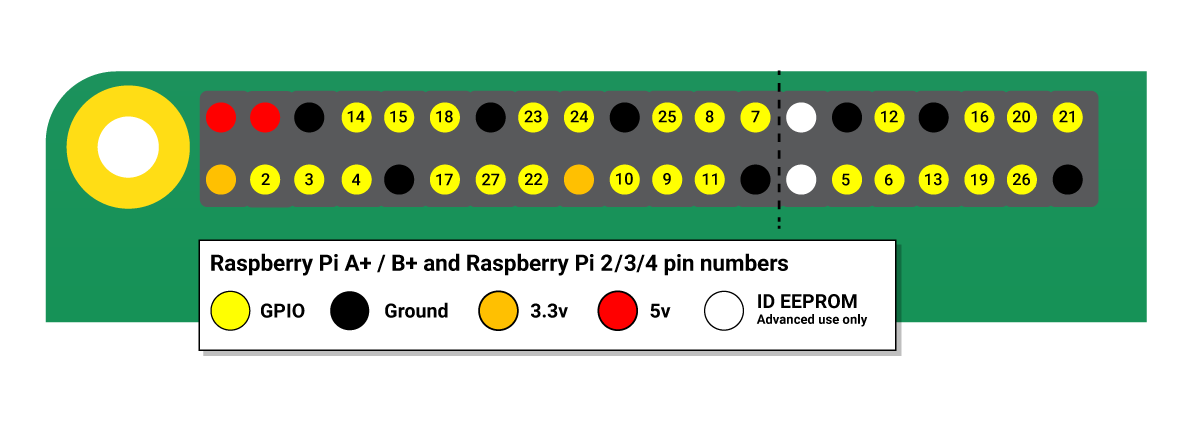
\includegraphics[width=0.7\textwidth]{figures/GPIO.png}
    \caption{Representação alternativa dos \acrshort{gpio}s \cite{Raspberrytech}}
    \label{fig:gpiocores}
\end{figure}

\subsection{Relés}
\label{sec:reles}
Como já foi referido na Capítulo \ref{Capitulo2}, os circuitos que compõem o \acrshort{visir} são controlados através de relés. Estes dispositivos funcionam como interruptores electromecânicos simples que utilizam um sinal elétrico para controlar um eletroíman.
Os relés electromecânicos são constituídos por uma bobine e um contacto, que pode ser normalmente aberto ou fechado. A corrente eléctrica ao passar pela bobine gera um campo magnético que atrai o contacto, fechando-o ou abrindo-o, conforme o caso. A Figura \ref{fig:esquematicoreles} mostra um esquema simplificado de um relé electromecânico.

\begin{figure}[hbtp]
    \centering
    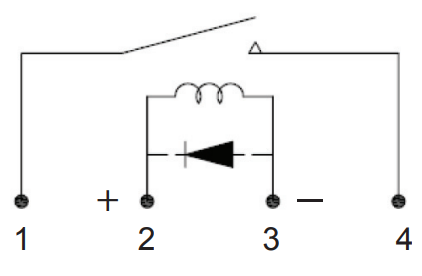
\includegraphics[width=0.3\textwidth]{figures/esquematico_rele.png}
    \caption{\textit{Esquema simplificado de um relé \cite{DryRelay}}}
    \label{fig:esquematicoreles}
\end{figure}

Ainda na Figura \ref{fig:esquematicoreles} pode ver-se a inclusão do díodo de ``roda livre'', que é comum em muitos relés. Este díodo é usado para proteger o circuito de comando de picos de tensão induzidos pela bobine do relé, quando a corrente é desligada, segundo a Lei de Faraday. O díodo permite que a corrente induzida pela bobine circule em circuito fechado, evitando danos no circuito comandados pelos relés.

Os relés utilizados no \acrshort{lare} estavam disponíveis em contexto laboratorial e são em tudo idênticos aos que se encontram montados no \acrshort{visir}  do \acrshort{isep}.

No \acrshort{lare} foram usados dois tipos de relés - simples, \acrfull{spst} e duplos, \acrfull{dpst}, como se pode ver na Figura \ref {fig:reles}.

Os modelos utilizados foram ambos da \textit{Comus}: relé \acrshort{spst}, ref. 3570-1331-123 e relé \acrshort{dpst}, ref. 3572-1220-123. As características mais importantes encontram-se descritas no \textit{datasheet} anexo a este documento. \textbf{Ver como fazer a referência ao datasheet}. Os dois primeiros quartetos indicam a série do relé e os três números indicam a tensão da bobine e a presença, ou não, do díodo de ``roda livre''. No caso dos relés usados, a tensão da bobine é de \SI{12}{\volt} e o díodo está ligado entre os pinos 2(+) e 6(-) \cite{DryRelay}. Tentou-se, sempre que possível, utilizar os relés \acrshort{spst} no comando das fontes e aparelhos de medida e os relés \acrshort{dpst} no controlo dos componentes. Serão devidamente referidos os casos em que isso não foi possível, por indisponibilidade dos componentes.

\begin{figure}[hbtp]
    \centering
    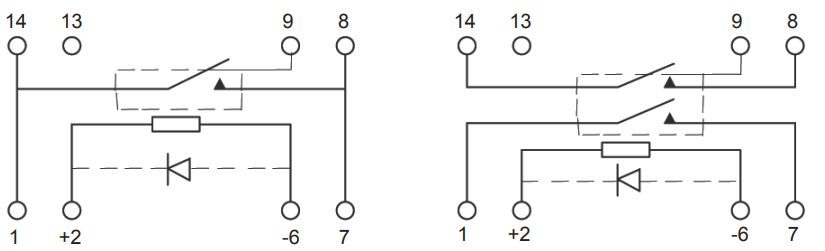
\includegraphics[width=0.5\textwidth]{figures/reles.png}
    \caption{\textit{Relés \acrshort{spst} e \acrshort{dpst}} \cite{DryRelay}}
    \label{fig:reles}
\end{figure}

Como já foi referido na Secção \ref{sec:RaspberryPI}, a tensão de funcionamento dos \acrshort{gpio}s, quer estejam configurados como entrada ou saída, é de \SI{3.3}{\volt}, sendo que a máxima corrente por cada \acrshort{gpio} é de \SI{16}{\mA}.
Com estes valores, o \gls{RaspberryPI} não tem capacidade para comandar os relés, já que funcionam a \SI{12}{\volt}. Para activar os relés, é necessário o uso de \textit{drivers}\footnote{Doravante, sempre que for referido o termo \textit{driver} no contexto de relés, subentende-se o circuito integrado \textit{ULN2003A}.} que consigam fornecer a tensão e corrente necessárias para o efeito.

\subsection{\textit{Driver} de Relés}
\label{sec:driver}
O circuito integrado ULN2003A é um \textit{driver} muito usado para controlar relés. Além disso estava disponível em contexto laboratorial.
Tipicamente, este \textit{driver} é usado em conjunto com microcontroladores ou \gls{RaspberryPI} no comando de cargas indutivas, como motores, bobines e relés.

Os ULN2003A possuem sete pares de transístores NPN, em configuração \textit{Darlington}, que apresentam saídas de alta tensão com díodos \textit{clamp} de cátodo comum para comutação de cargas indutivas \cite{ULN2003}, como se  representa esquematicamente na Figura \ref{fig:2003blocos}.

\begin{figure}[hbtp]
    \centering
    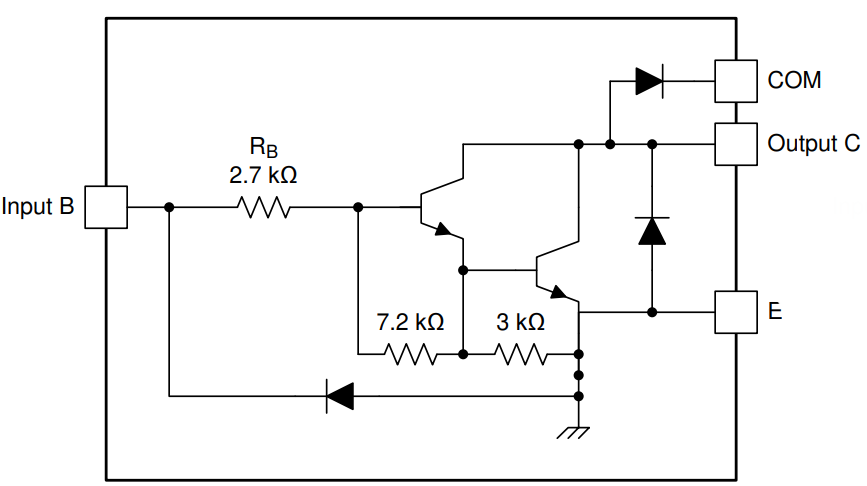
\includegraphics[width=0.5\textwidth]{figures/2003A_Darling.png}
    \caption{Diagrama de blocos ULN2003A \cite{ULN2003}}
    \label{fig:2003blocos}
\end{figure}

A corrente de colector de saída (única) é de \SI{500}{\mA} e a corrente de entrada, para uma tensão de entrada de \SI{3.85}{\volt}, é \SI{0.93}{\mA} \cite{ULN2003}.

Pela análise dos esquemas \textbf{DATASHEET - REFERÊNCIA} verifica-se que os \acrshort{gpio}s disponíveis no \gls{RaspberryPI} - 26 no total - não são suficientes para comandar os relés do \acrshort{lare}. Ao todo são utilizados 21 relés, o que corresponderia a 21 saídas. A experiência da Lei de Ohm, possui 8 relés. No caso das experiências correspondentes aos circuitos de rectificadores e filtros, o número de relés para efectuar as experiências é de 13. Falta adicionar os 10 \acrshort{gpio}s necessários para o controlo da transmissão das tramas de \textit{bits} \footnote{Este procedimento será abordado com mais \textbf{rigor, explicado melhor, blá, blá, nas secções seguintes - COLOCAR REFERÊNCIA}}.

Sendo assim, houve a necessidade de criar uma solução que permitisse comandar os relés, já que o \gls{RaspberryPI} não possui \acrshort{gpio}s suficientes.

\subsection{Registo de deslocamento}
\label{sec:registodeslocamento}
O uso de registos de deslocamento foi a solução encontrada de forma a ultrapassar o problema da falta de \acrshort{gpio}s.

O \textit{SN74HC595}\footnote{Doravante, sempre que for referido registo de deslocamento, subentende-se o circuito integrado \textit{SN74HC595}.} é um circuito integrado comum e bastante utilizado que contém um registo de deslocamento de 8 \textit{bits} com saídas \textit{3-State}, do tipo \acrfull{sipo}, que alimenta um registo de armazenamento do tipo D, também de 8 \textit{bits} e com saídas paralelas \textit{3-State}. O relógio para o registo de deslocamento e armazenamento é independente. A potência consumida é muito baixa, assim como a corrente de entrada \cite{SN74HC595}.

Descrição dos pinos de controlo:
\begin{itemize}
    \item \acrfull{ser}: é utilizado para enviar os \textit{bits} para o registo de deslocamento, um \textit{bit} de cada vez;

    \item \acrfull{srclk}: é o relógio do registo de deslocamento e é ativado no flanco ascendente, por cada impulso dado um \textit{bit} é enviado para o registo de deslocamento;

    \item \acrfull{rclk}: é o relógio do do registo de armazenamento e é activo no flanco ascendente. Quando activo, o conteúdo do registo de deslocamento é transferido para o registo de armazenamento, que eventualmente aparece na saída;

    \item \acrfull{srclr}: permite fazer o \textit{clear} ou \textit{reset} ao registo de deslocamento. Isto equivale a colocar todos os \textit{bits} a zero. Este pino é activo baixo.

    \item \acrfull{oe}: pino activo baixo que controla o estado da saída do registo: Se a zero as saídas estão activas, se a um as saídas estão desactivadas
\end{itemize}

Neste caso, os \textit{bits} são enviados um-a-um, armazenados no registo e depois enviados para a saída. A Figura \ref{fig:SN74HC595blocos} representa o diagrama de blocos do SN74HC595 e a Tabela \ref{Table:funcSN74HC595} representa os modos de funcionamento.

\begin{figure}[hbtp]
    \centering
    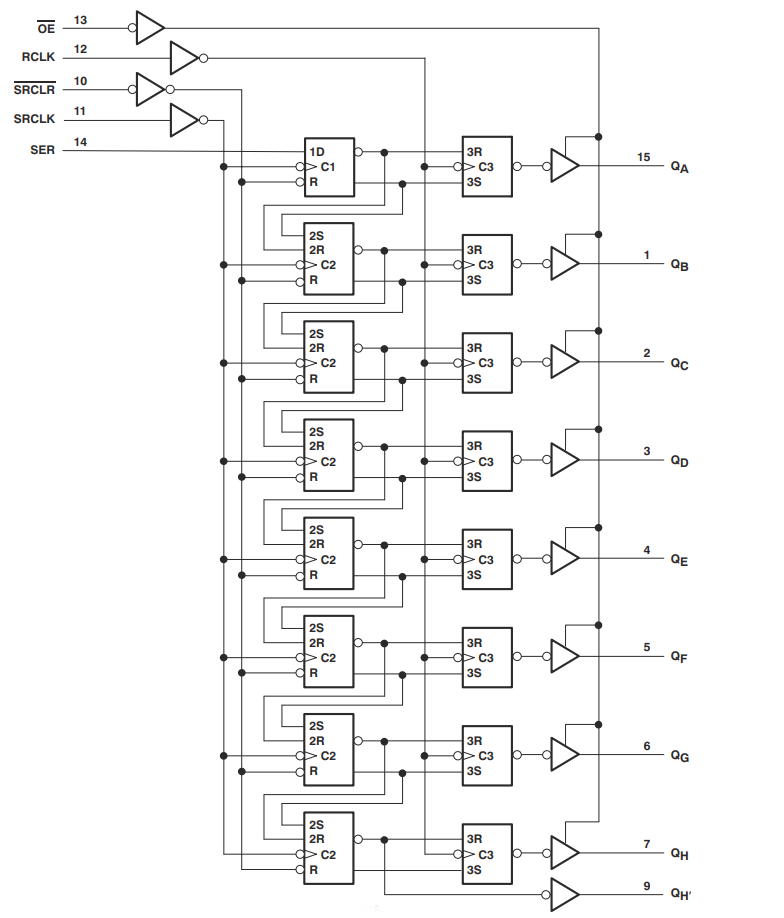
\includegraphics[width=0.7\textwidth]{figures/SR_blocos.png}
    \caption{Diagrama \textins{em corte} de blocos SN74HC595 \cite{SN74HC595}}
    \label{fig:SN74HC595blocos}
\end{figure}

Na transmissão das tramas optou-se por dividir as duas: envio de 8 \textit{bits}, na experiência da Lei de Ohm, e envio de 13 \textit{bits}, nas experiências de rectificadores e filtros. Como se pode ver na Tabela \ref{Table:funcSN74HC595}, são precisos 5 \acrshort{gpio}s configurados como saídas para controlar o envio de uma trama, portanto, para realizar o comando dos relés do \acrshort{lare}, são/serão necessários 10 \acrshort{gpio}s.
Nos capítulos seguintes - \textbf{COLOCAR A REFERÊNCIA} - é explicado com mais pormenor o processo de envio. As implicações ao nível do \textit{software} de programação são mínimas e ao nível do \textit{hardware} estão dentro dos limites de número de \acrshort{gpio}s do \gls{RaspberryPI}.

\begin{table}[htb]
    \caption{Modos de funcionamento do SN74HC595 \cite{SN74HC595}}
    \label{Table:funcSN74HC595}
    \resizebox{\textwidth}{!}{%
        \begin{tabular}{cccccl}
            \toprule
            \multicolumn{5}{c}{Entradas}           & \multicolumn{1}{c}{\multirow{3}{*}{Função}}                                                                                        \\
            \cline {1-5}
            \multicolumn{5}{l}{}                   &
            \multicolumn{1}{c}{}                                                                                                                                                        \\
            \multicolumn{1}{l}{SER}                &
            \multicolumn{1}{l}{SRCLK}              &
            \multicolumn{1}{l}{$\overline{SRCLR}$} &
            \multicolumn{1}{l}{RCLK}               &
            \multicolumn{1}{l}{$\overline{OE}$}    &
            \multicolumn{1}{c}{}                                                                                                                                                        \\
            \midrule
            X                                      & X                                           & X & X          & H & Saídas $Q_A$ – $Q_H$ estão desabilitadas.                       \\
            \midrule
            X                                      & X                                           & X & X          & L & Saídas $Q_A$ – $Q_H$ estão habilitadas.                         \\
            \midrule
            X                                      & X                                           & L & X          & X & Registo de deslocamento é limpo.                                \\
            \midrule
            L                                      &
            $\uparrow$                             &
            H                                      &
            X                                      &
            X                                      &
            \begin{tabular}[c]{@{}l@{}} Primeiro passo do registo de deslocamento vai a ``0''. \\ Passo seguinte armazena os dados do estado anterior, respectivamente. \end{tabular}   \\
            \midrule
            H                                      &
            $\uparrow$                             &
            H                                      &
            X                                      &
            X                                      &
            \begin{tabular}[c]{@{}l@{}}Primeiro passo do registo de deslocamento vai a ``1''. \\ Passo seguinte armazena os dados do estado anterior, respectivamente. \end{tabular}    \\
            \midrule
            X                                      & X                                           & X & $\uparrow$ & X & Os dados do registo de deslocamento são armazenados no registo. \\
            \bottomrule
        \end{tabular}%
    }
\end{table}

\textbf{Falta colocar informação complementar no datasheet em tal sítio está representada informação complementar respeitante ao ULN2003A e 74595}

\section{Software}
\label{sec:arquitecturasoftware} 
O \textit{software} do \acrshort{lare} foi dividido em duas grandes grupos/partes/secções(riscar o que não interessa): \textit{Back-end} e \textit{Front-end}.

Por \textit{Back-end} pode entender-se toda a programação e os processos a correr em segundo plano, que sustentam o funcionamento do \acrshort{lare}, incluindo servidor, \acrshort{api}s ou base de dados \cite{FrontbackEnd}. Existe uma grande variedade de linguagens de programação, \textit{frameworks} e ferramentas para realizar a gestão do \textit{Back-end}. Na implementação do \acrshort{lare}, utilizou-se o \textit{Python} como linguagem de programação e o \textit{Flask} como \textit{Framework}.

Já o \textit{Front-end} gere a parte do \textit{site}, isto é, a \textit{interface} com o utilizador e as aplicações que os utilizadores veem e com as quais interagem para realizar determinadas tarefas. As linguagens utilizadas na implementação do \textit{Front-end} para o \acrshort{lare} foram o \acrshort{html}, \acrfull{css} e \textit{JavaScript}. Enquanto o \acrshort{html} é a ``espinha dorsal'' estrutural de um \textit{site}, o \acrshort{css} lida com a aparência personalizada que define o estilo dos elementos visuais e o JavaScript afecta a forma como os elementos da página se movimentam \cite{FrontbackEnd}.

De uma forma resumida, o desenvolvimento de \textit{Front-end} refere-se ao lado do cliente (aspeto de uma página \textit{Web}) e o desenvolvimento de \textit{Back-end} refere-se ao lado do servidor (funcionamento de uma página \textit{Web}).

\subsection{\textit{Back-End}}
\label{sec:back-end}
\subsubsection{\textit{Python}}
O \textit{Python} é uma linguagem poderosa e fácil de aprender. Possui estruturas de dados de alto nível eficientes e uma abordagem simples, mas eficaz à programação orientada para objectos \cite{ThePython}. Apresenta, também, uma série de vantagens que se enquadram nos objectivos do desenvolvimento e implementação do \acrshort{lare} \cite{pythonvantagens}:
\begin{itemize}
    \item Curva suave de aprendizagem;
    \item Quantidade e variedade das bibliotecas;
    \item Portabilidade;
    \item Flexibilidade;
    \item Robustez;
    \item Suporte da comunidade.
\end{itemize}

Como desvantagens há a referir que, comparado com outras linguagens, o \textit{Python} é mais lento em termos de execução, já que é um tipo de linguagem de alto-nível, pelo que não é adaptado para aplicações móveis e consome mais recursos \cite{pythonvantagens} \cite{5MainDispython}.

Ainda assim, segundo a \textit{\href{https://spectrum.ieee.org/the-top-programming-languages-2023}{\textit{IEEE Spectrum}}} \cite{ieeespectrum}, o \textit{Python} foi considerada a linguagem mais popular em 2023.

\subsubsection{\textit{Flask}}
O \textit{Flask} é uma \textit{framework} leve e flexível para \textit{Python} que segue a filosofia \textit{UNIX} de ``fazer uma coisa bem feita''. A escolha do \textit{Flask} deveu-se, essencialmente, à facilidade de integração com o \textit{Python}, sendo uma das \textit{frameworks} mais populares em \textit{Python} \cite{Flask}. É uma \textit{framework} de aplicações \acrfull{wsgi} que descreve a forma como um servidor \textit{Web} comunica com aplicações \textit{Web} e como essas aplicações podem ser encadeadas para processar um pedido \cite{wsgi}. Depende, ainda do  \textit{Jinja}, que é um motor de criação de modelos que permite escrever código semelhante à sintaxe do \textit{Python}, de forma a renderizar o documento final \cite{Jinja}.

Tal como foi referido na Secção \ref{sec:contextualização}, foram ainda analisadas várias opções, incluindo a \textit{Django}, outra \textit{framework} bastante popular. Em \cite{Djangovsflask} e \cite{FlaskvsDjango}, por exemplo, é feita uma comparação exaustiva entre as duas \textit{frameworks}, não havendo uma decisão final sobre qual a melhor, mas sim sobre qual a que melhor se adapta às necessidades de implementação e desenvolvimento dos projectos.

No entanto, o \textit{Flask} foi concebido para tornar a iniciação rápida e fácil, com a capacidade de evoluir até aplicações mais complexas, sendo mais adapatado a pequenos projectos.

Pelas razões referidas anteriormente, e tendo em conta a análise feita aos prós e contras, considerou-se que tanto o \textit{Python} como o \textit{Flask} são as linguagens que melhor se enquadram e adaptam aos objectivos propostos para o \acrshort{lare}.

\subsection{Front-End}
\label{sec:frontend}
\subsubsection{\textit{Webpage}}
Como já foi referido na Secção \ref{sec:arquitecturasoftware}, o \textit{Front-end} diz respeito ao aspecto gráfico das páginas \textit{Web} e pretende-se que a prioridade na construção da página seja a simplicidade.

A escolha do desenvolvimento da página recaiu no \acrshort{html}, \acrshort{css} e (pontualmente - \textbf{REVER}) \textit{JavaScript}.

O \acrfull{w3c} é uma organização internacional que desenvolve padrões e diretrizes para a \textit{web} visando garantir que a esta permaneça aberta, acessível e interoperável para todos. Os principais objetivos são promover a compatibilidade entre diferentes sistemas e garantir que a \textit{web} seja acessível a todos os utilizadores, independentemente das suas capacidades ou dispositivos. O \acrshort{w3c} trabalha em várias áreas, incluindo \acrshort{html} e \acrshort{css} \cite{W3C}.

O \acrshort{html} é a linguagem \textit{standard}, usada para definir a estrutura do seu conteúdo e consiste numa série de elementos usados para delimitar ou agrupar diferentes partes do conteúdo. As \textit{tags} ou etiquetas, podem transformar uma palavra ou imagem num \textit{hyperlink}, pôr palavras em itálico, aumentar ou diminuir a fonte, etc. \cite{HTMLbasics}

Existem 3 tipos de elementos \cite{HTMLwikipedia}:
\begin{itemize}
    \item \textbf{Normais}: são elementos que têm uma etiqueta de abertura e outra de fecho. Por exemplo, <p></p> define um parágrafo;
    \item \textbf{Texto}: são elementos que não têm uma etiqueta de fecho. Por exemplo, <Title> especifica o título da página em texto simples;
    \item \textbf{Vazios}: têm somente uma etiqueta de início na forma de <tag>. Por exemplo, a etiqueta <img> referencia um ficheiro externo, neste caso uma imagem ou <br> que força uma quebra de linha.
\end{itemize}

Na Figura \ref{fig:estruturahtml} está representada a estrutura de uma página \acrshort{html}. De referir os navegadores não exibem as etiquetas HTML. O seu propósito é ler os documentos \acrshort{html} e apresentá-los corretamente.

\begin{figure}[hbtp]
    \centering
    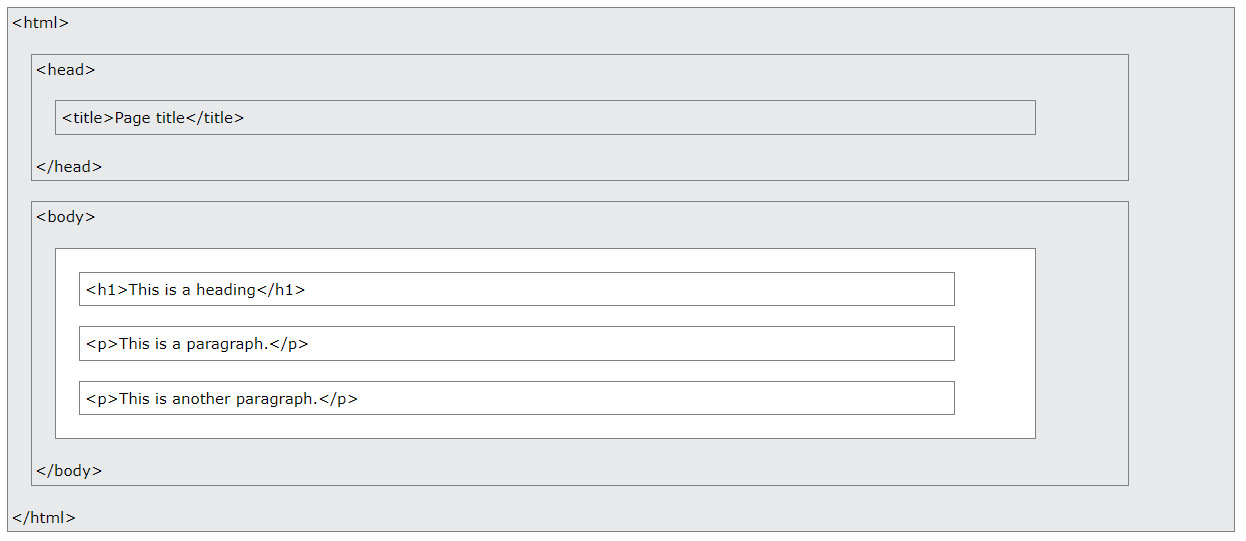
\includegraphics[width=0.7\textwidth]{figures/html_page_structure.png}
    \caption{Estrutura de uma página \acrshort{html} \cite{HTMLbasics}}
    \label{fig:estruturahtml}
\end{figure}

Segundo o consórcio \acrshort{w3c}, as \acrshort{css} são mecanismos fundamentais para a separação de preocupações no desenvolvimento \textit{web}. Ao delegar a responsabilidade de formatação visual no \acrshort{css}, o \acrshort{html} concentra-se na estrutura semântica do conteúdo. Isso resulta num código mais limpo, de fácil manutenção e acessível. As regras de estilo, que especificam como os elementos \acrshort{html} devem ser apresentados, podem ser aplicadas a elementos individuais, classes ou \textit{IDs}, permitindo um alto grau de customização. Além disso, o \acrshort{css} oferece a possibilidade de criar hierarquias de estilos, onde os mais específicos sobrepõem aos mais gerais. As folhas de estilo podem ser inseridas diretamente no documento \acrshort{html} ou vinculadas a ele através de um arquivo externo, proporcionando maior organização e reutilização de estilos \cite{w3ccss}.

Um exemplo simples pode ser visto na Listagem \ref{lst:excss}.

\begin{minipage}{0.9\linewidth}
    \begin{lstlisting}[language=HTML, caption=Exemplo \acrshort{css} incluído na página \acrshort{html} \cite{Startingcss}, label=lst:excss]
		<!DOCTYPE html PUBLIC "-//W3C//DTD HTML 4.01//EN">
		<html>
		<head>
		  <title>My first styled page</title>
		  <style type="text/css">
		  body {
			color: purple;
			background-color: #d8da3d }
		  </style>
		</head>
		
		<body>
		(...)
	\end{lstlisting}
\end{minipage}

As linhas 5 e 6 indicam que é uma folha de estilos escrita em \acrshort{css} e que o estilo está aplicado ao elemento \textit{body}. As linhas seguintes definem as cores do texto e fundo. No exemplo dado na Listagem \ref{lst:excss}, a folha de estilos está integrada directamente no ficheiro \acrshort{html}. Mas à medida que a página cresce em complexidade, torna-se incomportável manter a folha de estilos no ficheiro (ou ficheiros) \acrshort{html}. Para isso, cria-se a folha de estilos com a extensão \textit{.css} e referencia-se este ficheiro em todas as páginas. Neste caso, o exemplo da página apresentado na Listagem \ref{lst:excss} ficaria da forma apresentada na Listagem \ref{lst:paginahtmlcss}:

\begin{minipage}{0.9\linewidth}
    \begin{lstlisting}[language=HTML, caption=Exemplo da página \acrshort{html} com o \acrshort{css} definida externamente \cite{Startingcss}, label=lst:paginahtmlcss]
		<!DOCTYPE html PUBLIC "-//W3C//DTD HTML 4.01//EN">
		<html>
		<head>
		  <title>My first styled page</title>
		  <link rel="stylesheet" href="meuestilo.css">
		</head>
		
		<body>
		(...)
	\end{lstlisting}
\end{minipage}

Por sua vez, o ficheiro \textit{\textbf{meuestilo.css}} da forma apresentada na Listagem \ref{lst:cssexterno}:

\begin{minipage}{0.9\linewidth}
    \begin{lstlisting}[language=HTML, caption=Exemplo do \acrshort{css} definido externamente \cite{Startingcss}, label=lst:cssexterno]
		body {
			color: purple;
			background-color: #d8da3d }
		  </style>
		(...)
	\end{lstlisting}
\end{minipage}

No \href{https://jigsaw.w3.org/css-validator/}{link} e \href{https://validator.w3.org/}{link} é possível validar as folhas de estilo e as páginas \acrshort{html}, respectivamente.

Já o \textit{JavaScript} é uma linguagem de programação orientada para objectos e utilizada principalmente para \textit{scripts} dinâmicos do lado do cliente, permitindo que uma aplicação coloque elementos num formulário \acrshort{html} e responda a eventos do utilizador, como cliques do rato, preenchimento de formulários e navegação na página. Também pode ser utilizada no lado do servidor, permitindo que uma aplicação comunique com uma base de dados, mantenha a continuidade das informações entre diferentes chamadas da aplicação ou manipule ficheiro no servidor.

Isso significa que, no navegador, o \textit{JavaScript} pode alterar a aparência da página e, da mesma forma, o \textit{Node.js} - versão mais avançada do \textit{JavaScript} no servidor - pode responder a solicitações personalizadas enviadas pelo código executado no navegador.

Os programas nesta linguagem são chamados \textit{scripts}. Podem ser escritos directamente numa página \acrshort{html} e executados automaticamente quando a página é carregada. Estes \textit{scripts} são escritos e executados em texto simples e não precisam de compilador para correr.

O JavaScript pode ser executado não apenas nos navegadores, mas também nos servidores, ou, basicamente, em qualquer dispositivo que tenha um \textit{JavaScript Engine}, isto é, \textit{software} específico que execute o código \textit{JavaScript} \cite{JavaScriptRef}.

Na Listagem \ref{lst:exemplojava} está representado um exemplo de \textit{JavaScript} que desabilita os seletores de um formulário quando o botão ``OK'' é clicado.

\begin{minipage}{0.9\linewidth}
    \begin{lstlisting}[language=HTML, caption=Exemplo de \textit{JavaScript}, label=lst:exemplojava]
(...)
<script>
//Accionar a funcao habilitarSeletores quando o botao "OK" for clicado

document
  .querySelector(".stop")
  .addEventListener("click", desabilitarSeletores);
</script>
(...)
	\end{lstlisting}
\end{minipage}

Estas linguagens - \acrshort{html}, \acrshort{css} e \textit{JavaScript} - são interdependentes e frequentemente utilizadas em conjunto no desenvolvimento \textit{web}, cada uma desempenhando um papel específico na construção e estilização de páginas \textit{web} e na implementação de interatividade. Se o \acrshort{html} define o conteúdo das páginas, o \acrshort{css} define a sua aparência e o \textit{JavaScript} define o comportamento \cite{JavaScript}.


